\documentclass[a4paper,10pt, bibliography=totocnumbered]{scrreprt}

\usepackage[utf8x]{inputenc}
\usepackage[english]{babel}

\usepackage{graphicx}
\usepackage{pdfpages}
%\usepackage{subfig}
%\usepackage{microtype}
\usepackage{tabularx}
%\usepackage{amsmath, textcomp}

% Custom packages
\usepackage[numbers]{natbib}
\usepackage{longtable}
\usepackage{ragged2e}
%\usepackage{tikz}
%\usetikzlibrary{positioning}
%\usepackage{pdflscape}
%\usepackage{rotating}

\usepackage{glossaries} 

\usepackage{hyperref}
\hypersetup{
    colorlinks=true,        % false: boxed links; true: colored links
    linkcolor=black,        % color of internal links
%    citecolor=green,        % color of links to bibliography
    citecolor=black,        % color of links to bibliography
    filecolor=magenta,      % color of file links
    urlcolor=blue           % color of external links
}


%% Title Page
\makeatletter
\renewcommand{\maketitle}{\begin{titlepage}
    \vskip 10\p@
    \hbox{
      \vrule depth 0.99\textheight
        \mbox{\hspace{2em}}
      \vtop{
        \vskip 10\p@
        \hspace{4pt}
        \vskip 50\p@
        \begin{flushleft}
          \Large \@author \par
        \end{flushleft}
        \vskip 50\p@
        \begin{flushleft}
          \huge \bfseries \@title \par
        \end{flushleft}
        \begin{flushleft}
          \Large \bfseries \@subtitle \par
        \end{flushleft}
        \vskip 70\p@
        \begin{flushleft}
          \Large \@publishers \par
        \end{flushleft}
        \vskip 50\p@
        \begin{flushleft}
          \Large \@date \par
        \end{flushleft}
        }}
  \end{titlepage}
}
\makeatother

\author{Author 1, Author n}
\title{Title }
\subtitle{Technical Report}
\publishers{\textbf{Advisor University of Heidelberg}\\ Prof. Dr. Barbara Paech, Michael Anders}
\date{mm dd, year}



% Deutsche Absaetze:
\parindent 0pt
\parskip 12pt

\textwidth145mm
\setlength{\oddsidemargin}{0.7cm}
\setlength{\topmargin}{-0.5cm}
\setlength{\textheight}{22.5cm}

\begin{document}
\maketitle

\begin{abstract}
\section*{Abstract}
Place the abstract in this section.
\end{abstract}

\tableofcontents

\chapter{Introduction}
Lorem ipsum dolor sit amet, consectetuer adipiscing \textbf{Figure \ref{fig:model}} elit. Vivamus elementum sem eget tortor. Pellentesque id orci cursus sem tempus porttitor. Aenean tincidunt, neque vitae bibendum lacinia, magna erat dapibus nunc, vel pharetra nibh erat ac lorem. Ut suscipit ante eget magna. Morbi luctus aliquet odio. 

\section{Subsection}
Aenean turpis velit, ullamcorper sed, viverra vel, consectetuer sit amet, \cite{KunChen2005} Chenipsum. Phasellus sed lectus. Vivamus fermentum odio sed odio. Donec a dui. Duis et neque quis ligula pulvinar porttitor. Nunc mattis lectus vitae diam. 

Praesent quis orci. Aliquam id urna. Sed dolor erat, faucibus et, mattis eget, \textbf{commodo} nec, lorem. Etiam sit amet nisi sit amet nisi posuere bibendum. \emph{Cum sociis natoque} penatibus et magnis dis parturient montes, nascetur ridiculus mus. 


\begin{figure}
\centering
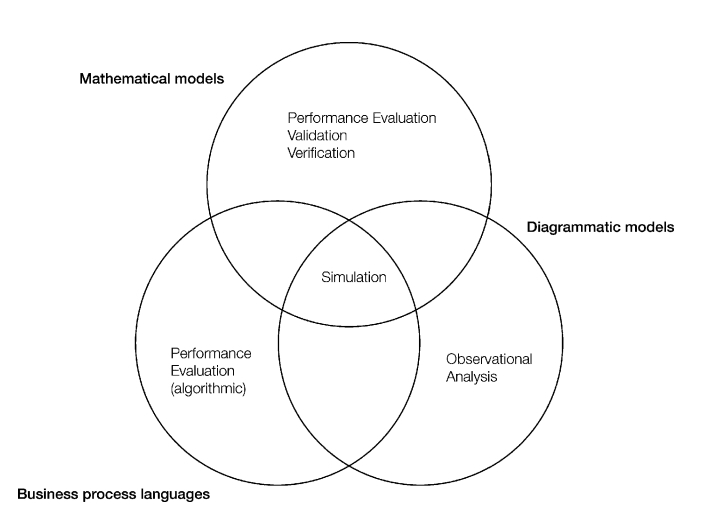
\includegraphics[scale=0.65]{images/T1Figure01.pdf} 
\caption{caption text}
\label{fig:model}
\end{figure}

\begin{itemize}
\item Aliquam
\item mus
\item montes
\end{itemize}

\subsubsection{Subsubsection}
Lorem ipsum dolor sit amet, consectetuer adipiscing elit. Vivamus elementum sem eget tortor. Pellentesque id orci cursus sem tempus porttitor. Aenean tincidunt, neque vitae bibendum lacinia, magna erat dapibus \textbf{Table \ref{tab:table}} nunc, vel pharetra nibh erat ac lorem. Ut suscipit ante eget magna. Morbi luctus aliquet odio. Aenean turpis velit, ullamcorper sed, viverra vel, 

 \begin{table} [t] 
\centering
\begin{small}
\caption{Table caption text}
\label{tab:table}
\setlength{\tabcolsep}{1em}
\begin{tabular}{ l| p{8cm}}
\hline
 \textbf{X} & \textbf{ Y} \\
\hline
 \hline	
 Item1 & description\\
 \hline
  Item2 & description  \\
 \hline
  Item2 & description \\
 \hline
\end{tabular}
\end{small}
\end{table}

\chapter{Richtiges Zitieren}

1.	Die Seminararbeit ist eine eigenständige wissenschaftliche Arbeit und wird auch nach den Regeln einer wissenschaftlichen Arbeit erstellt (vgl.~\cite{RichtigesZitierenTUDresden}), insbesondere heißt das, dass die Regeln für:
\begin{enumerate}
\item Richtiges Zitieren 
\begin{itemize}
\item Zitierpflicht
\item Zitierregeln
\item Typen von Zitaten
\item Zitierformen
\end{itemize}
\item Literaturangaben 
\item eine gut strukturierte Arbeit 
\end{enumerate}
beachtet und eingehalten werden.




\chapter{Chapter}

Duis porta orci. Integer eu arcu at enim tempus facilisis. Pellentesque dignissim orci sed est. Etiam elementum laoreet mi. Donec nunc sapien, dictum in, tristique sed, aliquam vitae, massa. Morbi magna magna, vestibulum tempor, lobortis non, convallis nec, nibh. In sed nibh. Suspendisse adipiscing dictum pede. Suspendisse non augue. Lorem ipsum dolor sit amet, consectetuer adipiscing elit. Pellentesque lacinia, velit sed commodo convallis, diam dolor consequat ligula, a scelerisque quam neque et purus. Praesent vel augue. Sed lectus leo, dignissim eget, vulputate eu, auctor ut, nulla. Vivamus a quam. Nulla tellus. Pellentesque tempor pulvinar nunc.


\chapter{Conclusion}
Fusce vitae quam eu lacus pulvinar vulputate. Suspendisse potenti. Aliquam imperdiet ornare nibh. Cras molestie tortor non erat. Donec dapibus diam sed mauris laoreet volutpat. Sed at ante id nibh consectetuer convallis. Suspendisse diam tortor, lobortis eget, porttitor sed, molestie sed, nisl. Integer enim nisl, lacinia in, pretium eu, viverra a, odio. Quisque at quam eget risus placerat porttitor. Suspendisse convallis, elit vitae mattis pharetra, orci nisl ultrices sapien, ac interdum metus lorem iaculis diam. Nunc id nunc sit amet nisl tincidunt congue. Curabitur et sapien.

%% Bibliography
\bibliographystyle{plainnat}
%\bibliography{literature.bib}%Bibliography file name

\begin{thebibliography}{9}

\bibitem{KunChen2005} Chen, K, Zhang, W., Zhao, H.: An approach to constructing feature models based on requirements clustering.
In: 13th IEEE International Conference on Requirements Engineering (RE05). pp. 31-40. (2005)

\bibitem{RichtigesZitierenTUDresden} Institut für Geographie   
Lehrstuhl für Allgemeine Wirtschafts- und Sozialgeographie: An Hinweise zum wissenschaftlichen Arbeiten.
\url{http://www.geogr.uni-jena.de/fileadmin/Geoinformatik/Lehre/backup_05_2007/pdf-dokumente/Skript_WissArbeiten.pdf}

% Sources Topic 2 Start
\bibitem{Ciurumelea.2017} A. Ciurumelea, A. Schaufelbühl, S. Panichella and H. C. Gall, "Analyzing reviews and code of mobile apps for better release planning" 2017 IEEE 24th International Conference on Software Analysis, Evolution and Reengineering (SANER), 2017, pp. 91-102, doi: 10.1109/SANER.2017.7884612.
  
\bibitem{Scalabrino.2019} S. Scalabrino, G. Bavota, B. Russo, M. D. Penta and R. Oliveto, "Listening to the Crowd for the Release Planning of Mobile Apps," in IEEE Transactions on Software Engineering, vol. 45, no. 1, pp. 68-86, 1 Jan. 2019, doi: 10.1109/TSE.2017.2759112.

\bibitem{Villarroel.2016}L. Villarroel, G. Bavota, B. Russo, R. Oliveto and M. Di Penta, "Release Planning of Mobile Apps Based on User Reviews," 2016 IEEE/ACM 38th International Conference on Software Engineering (ICSE), 2016, pp. 14-24, doi: 10.1145/2884781.2884818.
  
\bibitem{Mahmud.2019}O. Mahmud, N. T. Niloy, M. A. Rahman and M. S. Siddik, "Predicting an Effective Android Application Release Based on User Reviews and Ratings," 2019 7th International Conference on Smart Computing \& Communications (ICSCC), 2019, pp. 1-5, doi: 10.1109/ICSCC.2019.8843677.

\bibitem{Noei.2019}E. Noei, F. Zhang and Y. Zou, "Too Many User-Reviews! What Should App Developers Look at First?," in IEEE Transactions on Software Engineering, vol. 47, no. 2, pp. 367-378, 1 Feb. 2021, doi: 10.1109/TSE.2019.2893171.

\bibitem{Aslam.2020}N. Aslam, W. Y. Ramay, K. Xia and N. Sarwar, "Convolutional Neural Network Based Classification of App Reviews," in IEEE Access, vol. 8, pp. 185619-185628, 2020, doi: 10.1109/ACCESS.2020.3029634.

\bibitem{Suprayogi.2018}E. Suprayogi, I. Budi and R. Mahendra, "Information Extraction for Mobile Application User Review," 2018 International Conference on Advanced Computer Science and Information Systems (ICACSIS), 2018, pp. 343-348, doi: 10.1109/ICACSIS.2018.8618164.
% Sources Topic 2 End

\end{thebibliography}

\listoffigures

\listoftables

\end{document}          
